The \ac{KPN} model was defined by Gilles Kahn in 1974~\cite{kahn74}.
While in this paper he motivated examples of such networks could we defined, the
semantics of a concrete language to were only postulated by Kahn with MacQueen
in 1976~\cite{kahn_macqueen}.
However, there is a gap in the semantics of formally defined networks (\ac{KPN})
and the concrete networks that can be defined by the Kahn-MacQueen
blocking-reads execution semantics: These concrete semantics are not as general
as the formal model allows them to be.
More interestingly, there are networks which fall under the \ac{KPN} formalism
that cannot be expressed using the Kahn-MacQueen blocking-reads semantics.
We call this gap in the semantics ``the MacQueen gap'', as the gap between the formal model by Kahn and the concrete execution semantics by Kahn and MacQueen~\cite{lee_matsikoudis_semantics,,khasanov_parmaditam18}. 

In this Section we explore the MacQueen gap by showing the difference is between the two formalisms, and see how we can exploit it. The theoretical advantage from this semantics gap is the contribution of this thesis with regards to this subject. To better understand it, however, we also discuss the results of a practical implementation of a library implemented by Khasanov~\cite{khasanov_parmaditam18} that exploits this gap in the semantics. 

\subsection{The MacQueen Gap}

Recall the definition of a \ac{KPN} from~\ref{sec:mocs}.
A Kahn Process Network is a directed graph $K = (V,E)$ where the edges $V$ are Scott-continuous~\cite{scott1970} functions $f \in V$ mapping from the set of sequences from the input channels $S_{i_1} \times S_{i_k}$ to the set of output channels $S_{o_1} \times S_{o_l}$, and the edges represent the corresponding sequence domains.

Conversely, the Kahn-MacQueen blocking reads semantics are defined in a more operational fashion. The model of computation is defined implicitly by the semantics of a language\cite{kahn_macqueen}, characterized mainly through blocking reads to channels. While the original semantics by Kahn~\cite{kahn74} do suggest a programming paradigm similar to the Kahn-MacQueen blocking-read semantics, Kahn's original examples in a programing language made the waiting explicit in the program, not implicit in the read semantics. Neither paper aims to prove that the semantics emerging from the proposed languages correspond to the mathematical semantics of the networks in terms of Scott-continuous functions.

A central point of this distinction is the level at which these two semantics are defined: while the Kahn Process Network semantics are defined at a denotational level, the Kahn-MacQueen blocking-read semantics are operational in nature, and thus, more fine grained. This distinction is also crucial for understanding the semantics gap, since the gap itself is operational in nature as well. 

To understand the difference between the semantics we will first consider both from a denotational point of view. It is obvious that the basic semantics of the language describe a finite directed graph, and conversely, that any finite directed graph can be defined this way, by sequentially listing every node and all incoming and outgoing edges.
Thus, we can think of every Kanh-MacQueen process as a function $f$ mapping from the set of sequences from the input channels $S_{i_1} \times S_{i_k}$ to the set of output channels $S_{o_1} \times S_{o_l}$.
The pertinent question for characterizing Kahn-MacQueen processes is the continuity. 

\begin{theorem}
\label{thm:macqueen}
A Kahn-MacQueen process is Scott-continuous.
\begin{proof}
\todo{prove}
\end{proof}
\end{theorem}

\begin{cor}
\label{cor:macqueen}
Every Kahn-MacQueen Network is a Kahn Process Network.
\end{cor}

What about the converse implication? Can every Kahn Process Network be realized by a program following the Kahn-MacQueen blocking-reads semantics?
To understand the challenges this imposes, consider the network defined in Figure~\ref{fig:macqueen_counterexample}.
%\begin{minipage}
%\end{minipage}

\begin{figure}[h]
	%\centering
   \resizebox{0.85\textwidth}{!}{%inspired from: https://tex.stackexchange.com/questions/386345/directed-graph-example-in-tikz
\begin{tikzpicture}[
     > = stealth, % arrow head style
     shorten > = 1pt, % don't touch arrow head to node
     auto,
     node distance = 2cm, % distance between nodes
     semithick % line style
 ]

 \tikzstyle{process}=[
     draw = black,
     ellipse,
     thick,
     fill = white,
     minimum width = 3.5em,
     minimum height = 3.5em,
 ]
 \tikzstyle{mybox} = [
   very thick,
   rectangle,
   rounded corners,
   inner sep=10pt,
   inner ysep=20pt]

 \node[process] (s1) {\Large $s_1$};
 \node[process] (f) [below right of=s1] {\Large $f$};
 \node[process] (s2) [below left of=f] {\Large $s_2$};
 \node[process] (k) [right of=f] {\Large $k_1$};

 \path[->] (s1) edge node {\Large $i_1$}(f);
 \path[->] (s2) edge node {\Large $i_2$}(f);
 \path[->] (f) edge node {\Large $o_1$}(k);

 \node[mybox] (defn) [right of=k, node distance = 5cm] {
  \begin{minipage}{0.7\textwidth}
    \Large
   \begin{equation*}
     f : S_{i_1} \times S_{i_2} \rightarrow S_{o_1}  
   \end{equation*} 
   \begin{equation*}
     \begin{split}
     f : (x,y) = ((x_1,\ldots,x_j),(y_1,\ldots,y_k))  \\
     \mapsto (x_1+y_1,\ldots,x_{\min(j,k)}+y_{\min(j,k)})
     \end{split}
   \end{equation*}
  \end{minipage}
};
\end{tikzpicture}
}
	\caption{An example of a \ac{KPN} which admits non-blocking-read semantics.}
	\label{fig:macqueen_counterexample}
\end{figure}

By abuse of notation, we allow $j, k = \infty$ and for $j = \infty = k$ to mean that for two streams $x : \omega \rightarrow \Sigma_{i_1}, y : \omega \rightarrow \Sigma_{i_2}$ we define $f((x_i,y_i)) = (x_i+y_i)$ for all $i \in \mathbb{N}$.
The process $f$ is, thus, a deterministic merge via addition of the two input streams and obviously Scott-continuous, i.e. a Kahn process.

Now consider the following three cases:
\begin{enumerate}
\item $x = \epsilon, y = (1)$
\item $x = (1), y = \epsilon$
\item $x = (1), y = (1)$
\end{enumerate}

It is clear that the first two cases are prefixes of the third.
By the definition of $f$, only this third case will generate an output $(2)$, whereas the first two cases will result in an empty stream on the output channel $o_1$. 
However, operationally, there are different ways of processing these streams.
A Kahn-MacQueen program has to choose to read one channel first, blocking, then read the second channel, blocking, and then output the sum.
Listing~\ref{todo} shows an example of code in their original language proposed by Kahn and MacQueen.
\fbox{
Process F in I1,I2 out O1 ;
 Vars x,y ;
 repeat GET(I1) -> x; GET(I2) -> y; PUT(x+y,O1);
 forever
}

This implementation will block in Case 1 leaving unread data in channels, while it will execute normally in cases 2 and 3.
This is because we (arbitrarily) choose to read $i_1$ before $i_2$.
If we reverse this order, the implementation would block on Case 2 instead, leaving unread tokens in the channel $i_1$.
This is relevant if we consider the execution and communication times, since e.g. there is a finite read time required to read every channel. 
Consider the Gantt-charts depicted in Figure~\ref{fig:macqueen_example_gantt}. They show how blocking when reading $i_1$ delays the whole execution, even if $i_2$ could be read.
This is because the blocking-read semantics forces a deterministic ordering of reading tokens when executing, whereas the \ac{KPN} semantics only require the output to be deterministic, not the order of the computation itself.

\begin{figure}[h]
	%\centering
   \resizebox{0.85\textwidth}{!}{\begin{ganttchart}{1}{14}
  \gantttitle{Read $1$ first}{14} \\
  \ganttbar{Read $i_1$}{4}{6} \\
  \ganttbar{Read $i_2$}{7}{9} \\
  \ganttbar{execute $+$}{10}{11} \\
  \ganttbar{Write $o_1$}{12}{13}
  \ganttvrule{$i_2 = 1$}{1}
  \ganttvrule{$i_1 = 1$}{3}
  %\ganttvrule[vrule/.append style={red, thin},vrule offset=.2,23 vrule label node/.append style={anchor=north west}]{day z}{6}\
%  \ganttlink{elem1}{elem2}
%  \ganttlink{elem1}{elem3}
%  \ganttlink{elem2}{elem3}
%  \ganttlink{elem3}{elem4}
  \end{ganttchart}

\begin{ganttchart}{1}{14}
  \gantttitle{Read $2$ first}{14} \\
  \ganttbar{Read $i_1$}{5}{7} \\
  \ganttbar{Read $i_2$}{2}{4} \\
  \ganttbar{execute $+$}{8}{9} \\
  \ganttbar{Write $o_1$}{10}{11}
  \ganttvrule{$i_2 = 1$}{1}
  \ganttvrule{$i_1 = 1$}{3}
  \end{ganttchart}
}
	\caption{Examples of Gantt Charts corresponding to implementations of the Kahn Function $f$.}
	\label{fig:macqueen_example_gantt}
\end{figure}

Having understood the nature of the semantics gap, we can thus return to the question of the other direction in Theorem~\ref{thm:macqueen}.
The gap we have shown here exposes a difference in the operational semantics, yet the different versions discussed all result in the same denotational Kahn process as defined in Figure~\ref{fig:macqueen_counterexample}.
This does not contradict the converse direction to Theorem~\ref{thm:macqueen}.

\begin{figure}[h]
	%\centering
   \resizebox{0.85\textwidth}{!}{\usetikzlibrary{arrows, automata}
%inspired from: https://tex.stackexchange.com/questions/386345/directed-graph-example-in-tikz
\begin{tikzpicture}[
     > = stealth, % arrow head style
     shorten > = 1pt, % don't touch arrow head to node
     auto,
     node distance = 2cm, % distance between nodes
     semithick % line style
 ]

 \tikzstyle{every state}=[
     draw = black,
     thick,
     fill = white,
     minimum size = 4mm
 ]
 \tikzstyle{mybox} = [
   very thick,
   rectangle,
   rounded corners,
   inner sep=10pt,
   inner ysep=20pt]

 \node[state] (s1) {$s_1$};
 \node[state] (g) [below right of=s1] {$g$};
 \node[state] (s2) [below left of=g] {$s_2$};
 \node[state] (k1) [above right of=g] {$k_1$};
 \node[state] (k2) [below right of=g] {$k_2$};

 \path[->] (s1) edge node {$i_1$}(g);
 \path[->] (s2) edge node {$i_2$}(g);
 \path[->] (f) edge node {$o_1$}(k1);
 \path[->] (f) edge node {$o_2$}(k2);

 \node[mybox] (defn) [right of=k, node distance = 4cm] {
  \begin{minipage}{0.5\textwidth}
   \begin{equation*}
     g : S_{i_1} \times S_{i_2} \rightarrow S_{o_1}  \times S_{o_2}
   \end{equation*} 
   \begin{equation*}
     g : (x,y) = (y,x)
   \end{equation*}
  \end{minipage}
};
\end{tikzpicture}
}
	\caption{A counterexample of the equivalence of Kahn-MacQueen and Kahn processes.}
	\label{fig:macqueen_proper_counterexample}
\end{figure}

By exploiting the problem exposed in the first example, we can come up with a proper counterexample to the reverse direction of Theorem~\ref{thm:macqueen}.
The example depicted in Figure~\ref{fig:macqueen_proper_counterexample} is again clearly a Kahn process (Scott continuous), which just forwards the two incoming channels independently.
In practice, this Kahn process is not very useful, but it serves formally as a simple counterexample to the equivalence of Kahn-MacQueen blocking-reads processes and Kahn processes.
To this, consider again as inputs streams $(i_1,i_2)$ the three cases from the first example: 
\begin{enumerate}
\item $x = \epsilon, y = (1)$
\item $x = (1), y = \epsilon$
\item $x = (1), y = (1)$
\end{enumerate}

Unlike $f$, $g$ has a different behavior for every case:
\begin{enumerate}
\item $g(\epsilon,1) = (1,\epsilon)$
\item $g(1,\epsilon) = (\epsilon,1)$
\item $g(1,1) = (1,1)$
\end{enumerate}

This process cannot be realized by a Kahn-MacQueen process with blocking reads. Assume there was such a process. Then, from the sequentiality of code, either $i_1$ or $i_2$ will be read first. Without loss of generality let us assume that $i_1$ is read first. Then for the input stream $(\epsilon,1)$ however, the process will block and will never output the $1$ from channel $i_2$, which yields the contradiction.


\subsection{Exploting the Gap}
We have seen in the previous section how there is a gap in the operational blocking-read semantics proposed by Kahn and MacQueen and the denotational \ac{KPN} semantics. While the counterexample from Figure~\ref{fig:macqueen_proper_counterexample} does not seem very useful, the gap in the operational nature shown in Figure~\ref{fig:macqueen_example_gantt} readily suggests how this gap could be exploited.
In general, the Scott continuity of \acp{KPN} requires the arrival of tokens to be determistic, but it does not require the execution of independent nodes to follow the same order as the tokens, as required by the Kahn-MacQueen blocking-read semantics. Thus, as suggested by the example, the MacQueen gap can be exploited for asynchronous computation, as long as it does not break determinism.

This asynchronous execution can be used to execute multiple workers in a data-parallel fashion.
Figure~\ref{fig:data_parallel_kpn} shows an example of a network which does this.
\begin{figure}[h]
	%\centering
   \resizebox{0.45\textwidth}{!}{%inspired from: https://tex.stackexchange.com/questions/386345/directed-graph-example-in-tikz
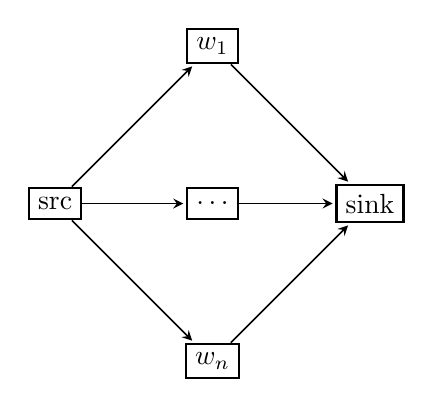
\begin{tikzpicture}[
     > = stealth, % arrow head style
     shorten > = 1pt, % don't touch arrow head to node
     auto,
     node distance = 2cm, % distance between nodes
     semithick % line style
 ]

 \tikzstyle{process} = [
     %cicrle,
     draw = black,
     thick,
     fill = white,
     minimum size = 4mm
 ]
 \tikzstyle{dots} = [
     draw = black,
     thick,
     fill = white,
     minimum size = 4mm
 ]

 \node[process] (src) {src};
 \node[dots] (wdots) [right of=src] {$\ldots$};
 \node[process] (wn) [below of=wdots] {$w_n$};
 \node[process] (w1) [above of =wdots] {$w_1$};
 \node[process] (sink) [right of=wdots] {sink};

 \path[->] (src) edge node {}(w1);
 \path[->] (src) edge node {}(wdots);
 \path[->] (src) edge node {}(wn);
 \path[->] (w1) edge node {}(sink);
 \path[->] (wdots) edge node {}(sink);
 \path[->] (wn) edge node {}(sink);
\end{tikzpicture}
}
	\caption{An example of data-parallelism exploiting the MacQueen gap.}
	\label{fig:data_parallel_kpn}
\end{figure}

The worker processes $w_1, \ldots, w_n$ can exploit data parallelism by dividing a workload into different parts. This allows us to asynchronously execute the workloads, as long as we take care to preserve the order at the sink node. 
We can achieve this by making it part of the logic of the channels. In joint work with R. Khasanov we proposed to exploit this gap and tested an implementation of this in the SLX framework which modified the FIFO libraries of nodes labeled as data-parallel to relax the deterministic semantics of the Kahn-MacQueen blocking-reads and allowed asynchronous execution of data-parallel workers while preserving the deterministic \ac{KPN} execution~\cite{khasanov_parmaditam18}. The implementation of this library is beyond the contribution of this thesis, which is limited to the theoretical part of identifying the semantics gap and ways of exploiting it.  

\todo{Question: Should I nevertheless discuss some results?}
